%-------------------------
% Resume in Latex
% Template: Sourabh Bajaj
% Author: Lukas Grams
% License : MIT
%------------------------

\documentclass[letterpaper,11pt]{article}

\usepackage{latexsym}
\usepackage[empty]{fullpage}
\usepackage{titlesec}
\usepackage{marvosym}
\usepackage[usenames,dvipsnames]{color}
\usepackage{verbatim}
\usepackage{enumitem}
\usepackage{xcolor}
\usepackage[colorlinks=true, urlcolor=blue, pdfborderstyle={/S/U/W 1},pdfborder=0 0 1, urlbordercolor=blue ]{hyperref}
%\usepackage[hidelinks]{hyperref}
%\usepackage{hyperref}
\usepackage{fancyhdr}
\usepackage{nccfoots}
\usepackage{graphicx}
\graphicspath{{C:/Users/GSYS/Downloads/} }
\usepackage{float}


\pagestyle{fancy}
\fancyhf{} % clear all header and footer fields
\fancyfoot{}
\renewcommand{\headrulewidth}{0pt}
\renewcommand{\footrulewidth}{0pt}

% Adjust margins
\addtolength{\oddsidemargin}{-0.5in}
\addtolength{\evensidemargin}{-0.5in}
\addtolength{\textwidth}{1in}
\addtolength{\topmargin}{-.5in}
\addtolength{\textheight}{1.0in}

\urlstyle{same}

\raggedbottom
\raggedright
\setlength{\tabcolsep}{0in}

% Sections formatting
\titleformat{\section}{
  \vspace{-4pt}\scshape\raggedright\large
}{}{0em}{}[\color{black}\titlerule \vspace{-5pt}]

%-------------------------
% Custom commands
\newcommand{\resumeItem}[2]{
  \item\small{
    \textbf{#1}{: #2 \vspace{-2pt}}
  }
}

\newcommand{\resumeItemWithoutHeadline}[1]{
	\item\small{
		{#1 \vspace{-2pt}}
	}
}

\newcommand{\resumeSubheading}[4]{
  \vspace{-1pt}\item
    \begin{tabular*}{0.97\textwidth}[t]{l@{\extracolsep{\fill}}r}
      \textbf{#1} & #2 \\
      \textit{\small#3} & \textit{\small #4} \\
    \end{tabular*}\vspace{-5pt}
}

\newcommand{\resumeSubItem}[2]{\resumeItem{#1}{#2}\vspace{-4pt}}

\renewcommand{\labelitemii}{$\circ$}

\newcommand{\resumeSubHeadingListStart}{\begin{itemize}[leftmargin=*]}
\newcommand{\resumeSubHeadingListEnd}{\end{itemize}}
\newcommand{\resumeItemListStart}{\begin{itemize}}
\newcommand{\resumeItemListEnd}{\end{itemize}\vspace{-5pt}}

%-------------------------------------------
%%%%%%  CV STARTS HERE  %%%%%%%%%%%%%%%%%%%%%%%%%%%%

\begin{document}

%----------HEADING-----------------
\begin{tabular*}{\textwidth}{l@{\extracolsep{\fill}}r}
	\textbf{\Large Lukas Grams}\\
	{geboren am 20.09.1994 in Düsseldorf}\\
	{Wohnort: Rosenheim, Bayern}\\
	{Tel : +49 151 6519 6156}\\  
	\big[
	\href{https://www.xing.com/profile/Lukas_Grams/cv}{Xing},
	\href{https://github.com/gramsimamsi/}{github},
	\href{https://www.linkedin.com/in/lukas-grams/?locale=de}{linkedin (de)},
	\href{https://www.linkedin.com/in/lukas-grams/?locale=en_US}{linkedin (en)} 
	\big] 
	\vspace*{-2.6cm}	\\
	Email : \href{mailto:lukas.grams.info@gmail.com}{lukas.grams.info@gmail.com} &
	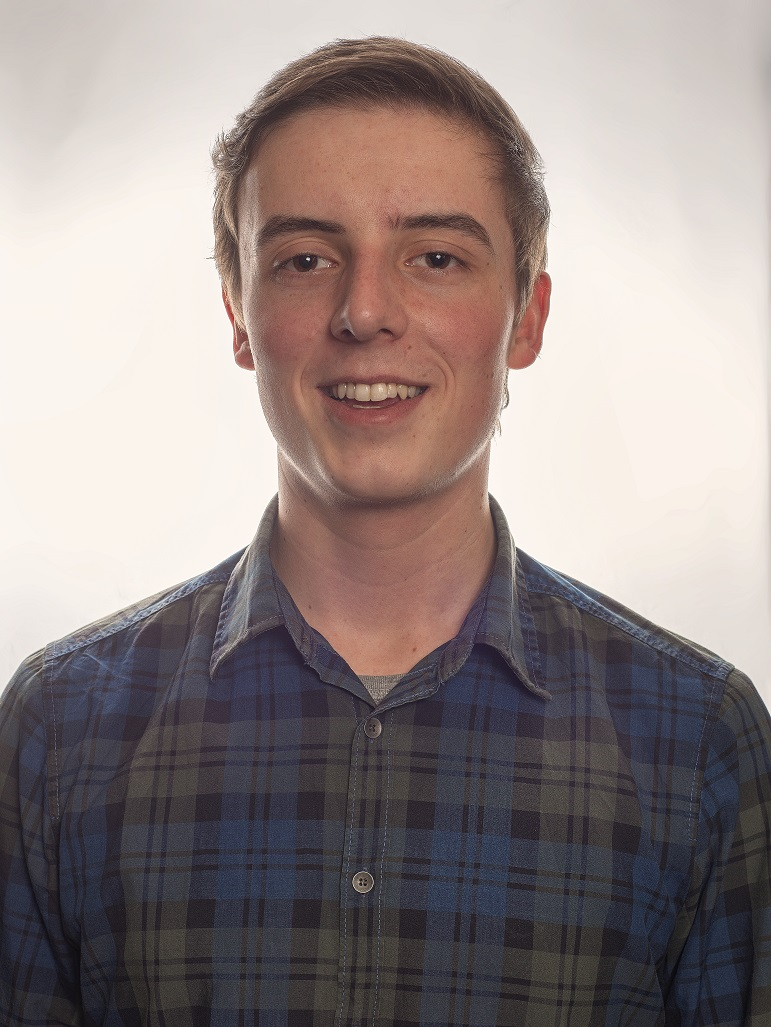
\includegraphics[scale=0.35]{Passbild.jpg}\\	
\end{tabular*}


%-----------EDUCATION----------------
\section{Ausbildung}
  \resumeSubHeadingListStart
    \resumeSubheading
   	  {B. Sc. Informatik}{2015 -- 2019}    
      {Hochschule Rosenheim,  Notenschnitt: 1,6}{Rosenheim}
    \resumeSubheading
      {Berufsausbildung IT-Systemelektroniker (IHK)}{2011 -- 2014}
      {Berufsschule München,  Notenschnitt: 1,0}{München}
  \resumeSubHeadingListEnd

%-----------EXPERIENCE-----------------
\section{Berufserfahrung}
  \resumeSubHeadingListStart
  
	\resumeSubheading
	{Junior Pentesting, Security Consultant}{2019 -- heute}
  	{Atos Information Technology Solutions}{München}
  	\resumeItemListStart
		\resumeItemWithoutHeadline
       	{Eigenständiges Planen und Durchführen von Penetrationstests mit und für Kunden der Atos \linebreak
       	mit Fokus auf Webapplikationen und Container-Umgebungen}
	\resumeItemListEnd
	
	\resumeSubheading
	{Werkstudent Junior IT Security Consultant}{2019}
  	{HvS-Consulting}{Garching}
  	\resumeItemListStart
		\resumeItemWithoutHeadline
       	{Operativer Einsatz in den Themengebieten Penetrationstest und Social Engineering}
	\resumeItemListEnd
	
	\resumeSubheading
	{Technical Specialist im Vulnerability Management}{2018}
	{Fujitsu Technology Solutions}{München}
	\resumeItemListStart
		\resumeItemWithoutHeadline
		{Entwickeln von Tools, Systemen und Prozessen zur Automatisierung \linebreak
		von Vulnerability Management Analysen und Alertings}
		\resumeItemWithoutHeadline
		{Verwendete Technologien: Docker, Git/GitLab, Ruby, Shell-Scripts, Ubuntu, RHEL, \linebreak
		Elasticsearch, Logstash, Kibana, Kolide Fleet, Osquery}
	\resumeItemListEnd

	\resumeSubheading
	{Tutor/Übungsleiter für Studienmodule}{2017 - 2018}
	{Hochschule Rosenheim, Fakultät Informatik}{Rosenheim}
	\resumeItemListStart
		\resumeItemWithoutHeadline
		{Programmieren 2: \linebreak
			Anleiten und Beraten der Studenten in fortgeschrittenen Konzepten der objektorientierten Programmierung \linebreak
			(Java, Funktionale Programmierung, Generics, Parallelisierung, Design Pattern) 
		}
		\resumeItemWithoutHeadline
		{Algorithmen \& Datenstrukturen: \linebreak
			Vermitteln von Modulinhalten und Klärung individueller Fragestellungen 	\linebreak
			zur Optimierung von Such- und Sortier-Algorithmen sowie den dazugehörigen Datenstukturen \linebreak
			(O-Komplexitätsanalysen, Heaps, Stacks, Baumstrukturen, Graphensuchen)
		}
	\resumeItemListEnd

	\resumeSubheading
	{Studentischer Mitarbeiter im \href{http://www.fh-rosenheim.de/forschung-entwicklung/kompetenzfelder-und-projekte/information-und-kommunikation/lv-selbstlernend/}{Forschungsprojekt "LV-selbstlernend"}}{2017}
	{Hochschule Rosenheim, Forschung \& Entwicklung}{Rosenheim}
	\resumeItemListStart
		\resumeItemWithoutHeadline
		{Entwicklung eines Softwaremoduls zum Auslesen von Sensordaten durch einen Raspberry Pi}
		\resumeItemWithoutHeadline
		{Modul-Auswahl und Design des Hardware-Systems}
		\resumeItemWithoutHeadline
		{Aufbau und Funktionstest eines Testsystems}
	\resumeItemListEnd
	
  \resumeSubHeadingListEnd

%--------Projects------------
\section{Projekte}
\resumeSubHeadingListStart
\item{
	\textbf{\href{https://github.com/gramsimamsi/bachelorThesis/blob/master/thesis.pdf}{Bachelorarbeit}}{: 	\linebreak 
		Identifizieren und Bewerten von Angriffsvektoren und Verteidigungsmaßnahmen in verteilten Container-Umgebungen sowie
		Ableitung von Maßnahmen zum priorisierten Risiko-Management auf Basis von
		Docker, Kubernetes, OpenShift, Azure, RHEL }
}
\item{
	\textbf{Privatprojekt Connected Home}{: 	\linebreak 
		Privates Docker-Setup für AdBlocking, VPN, Passwort-Manager und Medien-Streaming \linebreak
		aus Raspberry Pi, HypriotOS, Docker, PiHole, openVPN, KeePass, OpenPHT}
}
\item{
	\textbf{Studien-Projekt \href{https://github.com/gramsimamsi/thirstygames}{Thirstygames}}{: 	\linebreak 
		Tracken, kumulieren und Präsentieren von kompetitivem, team-basiertem \linebreak
		Zuführen überwiegend Hopfen-basierter Getränke. \linebreak 
		Entwicklung einer responsiven Web-App in 3-köpfigem Team unter Einsatz von \linebreak
		Angular 7, Material Design, ChartsJs, Express, Docker und Nginx }
}
\item{
	\textbf{Privatprojekt OSC-Exploit}{: 	\linebreak 
		Analysieren und Aushebeln des Notenbericht-Systems der TH Rosenheim - zu Weiterbildungszwecken	\linebreak
		Auswirkung: Einsicht der eigenen Prüfungsergebnisse vor offizieller Notenbekanntgabe.}
}
\item{
	\textbf{Projekt CowTracking}{: 	\linebreak 
		Orten von Kühen mithilfe einer LoRa-fähigen Full-Stack-Anwendung \linebreak
		bestehend aus Microcontroller, Backend-, DB- und Frontend-Servern, \linebreak
		Präsentieren des Projekts vor 
		\href{https://www.youtube.com/watch?v=JIbElz2qEes}{Großpublikum}
		und \href{https://www.rfo.de/mediathek/video/digitalisierungsmesse-an-der-hochschule-rosenheim/}{Presse} }
}
\item{
	\textbf{Studien-Projekt BSHolo}{: 	\linebreak 
		Anleiten eines 5-köpfigen Programmierer-Teams im \linebreak
		Entwickeln einer Hololens Augmented Reality Application für die Firma Bosch Siemens Haushaltsgeräte, \linebreak 
		Präsentieren des Projekts vor Großpublikum und \href{https://www.rfo.de/mediathek/video/projektmesse-an-der-hochschule-rosenheim/}{Presse} }
}
\item{
	\textbf{Privatprojekt Home-Audio}{: 	\linebreak 
		Netzwerkfähiges HiFi-Audiosystem \linebreak
		aus Raspberry Pi, DAC-Shield, Audiostream-Webserver und aktiven XLR-Boxen}
}
\resumeItemListEnd
%-------------------------------------------

%-----------VOLUNTEERING-----------------
\section{Ehrenamt}
  \resumeSubHeadingListStart  
  	
  	\resumeSubheading
  	{OWASP-Mitglied}{2018 - heute}
  	{Open Web Application Security Project}{}
  	\resumeItemListStart
  		\resumeItemWithoutHeadline
  		{Regelmäßiger Teilnehmer der Münchner OWASP-Stammtische}
  	\resumeItemListEnd
  
	\resumeSubheading
	{Semestersprecher und aktives Fachschaftsmitglied}{2015 - 2019}
	{Hochschule Rosenheim, Fakultät Informatik}{Rosenheim}
	\resumeItemListStart
		\resumeItemWithoutHeadline
		{Bilaterale Interessenvertretung von Studenten und Professoren}
		\resumeItemWithoutHeadline
		{Organisation von Informationsabenden, Festen und weiteren Aktionen}
	\resumeItemListEnd
	
	\resumeSubheading
	{Aktiver Mitarbeiter in ehrenamtlicher Kinder- und Jugend-Betreuung}{2015 - 2017}
	{Jugendwerk Rosenheim}{Rosenheim}
	\resumeItemListStart
		\resumeItemWithoutHeadline
		{Aus- und Weiterbildung angehender und amtierender Jugendleiter}
		\resumeItemWithoutHeadline
		{Konzeptionelle Ausrichtung und Budgetplanung der ehrenamtlichen Einrichtung}
		\resumeItemWithoutHeadline
		{Planen und Durchführen von Schulungen, Tages- und Wochenend-Aktionen}
	\resumeItemListEnd
	
  \resumeSubHeadingListEnd

%--------SKILLS------------
\section{Gemischtes}
\resumeSubHeadingListStart
\item{
	\textbf{Sprachen}{: 	
		\resumeItemListStart
		\resumeItemWithoutHeadline
		{Deutsch: Muttersprache}
		\resumeItemWithoutHeadline
		{Englisch: präsentations- und verhandlungssicher, fließend in Wort und Schrift}
		\resumeItemListEnd
}}
\item{
	\textbf{Events}{: 	
		\resumeItemListStart
		\resumeItemWithoutHeadline
		{Teilnahme an CTF-Challenges (Cyber Security Rumble, Reply Cyber Security Challenge)}
		\resumeItemWithoutHeadline
		{Regelmäßige Teilnahme an Meetups (Docker Workshops, Startup Incubator Stellwerk18)}
		\resumeItemListEnd
}}
\item{
	\textbf{Fachvorträge}{: 
		\resumeItemListStart
		\resumeItemWithoutHeadline
		{Entwerfen und Abhalten von Docker-Einführungs-Workshops}
		\resumeItemWithoutHeadline
		{Einführungen für zukünftige und startende Informatik-Studierende}
		\resumeItemListEnd
}}
\resumeSubHeadingListEnd
%-----------------------------

\raggedleft 
\tiny{Dieser Lebenslauf ist in LaTeX geschrieben. Der Sourcefile ist auf meinem \href{https://github.com/gramsimamsi/resume/blob/master/lukas_grams_resume.tex}{github repository} zu finden. }
\end{document}
